\documentclass[utf8, 11pt]{feuille}

\newcommand{\titredutd}{\textbf{Contrôle continu de 2 h 30 --- Mercredi 14 décembre 2022}}

\begin{document}

Seules les calculatrices non communicantes, les notes manuscrites personnelles, les dictionnaires de langues sont autorisées. Les exercices sont totalement indépendants. 

On notera $k_B$ la constante de Boltzmann et $h$ la constante de Planck.



%__________________________________________________________________________________


\section{Température de Fermi de l'argent (28 points)}

On considère un système de fermions libres et indépendants confinés à la température $T$ et au potentiel chimique $\mu$ dans un volume $V$. Dans l'approximation d'un continuum d'états quantiques individuels, on introduit $\rho(\epsilon)$ la densité d'états en énergie ($0\le \epsilon < +\infty$).

\question Exprimer sous forme d'une intégrale sur l'énergie, le nombre moyen de particules $\langle N \rangle$, l'énergie moyenne $U$ et le grand potentiel $J$.

\question On fait l'hypothèse que $\rho(\epsilon)$ est de la forme $A\epsilon^p$ ($p >0$). Montrer en effectuant une intégration par partie judicieuse que $J=-\frac{U}{p+1}$.

Comme la plupart des métaux usuels, l’argent solide libère un électron de conduction par atome. On considère un volume $V$ d’argent solide contenant un nombre $N$ d’atomes. On donne la masse atomique de l'argent: 108 g.mol$^{-1}$; la masse volumique de l'argent: 10,5 g.cm$^{-3}$; la masse de l'électron : 9,1 $\times 10^{-31}$ kg.

\question Calculer la densité de particules $n=\frac{N}{V}$ de l'argent solide.


\question On rappelle qu'à trois dimensions, la densité d'état d'un gaz parfait de fermions de spin $1/2$ et de masse $m$ est égale à $\rho(\epsilon)=\frac{V}{2\pi^2}(\frac{2 m}{\hbar^2})^{\frac{3}{2}} \sqrt{\epsilon}$. \'Etablir l’expression de la température de Fermi $T_F$ du gaz formé par les électrons de conduction supposés sans interaction en fonction de $n$ et des données. 

\question Calculer l’ordre de grandeur de $T_F$ pour l’argent. Quelle est l’importance physique de ce résultat ?  Peut-on traiter les électrons d'un métal avec la statistique de Maxwell-Boltzmann à température ambiante ?

\question \'Etablir  l’expression de la pression $P$ de ce gaz de Fermi à température nulle. Calculer l’ordre de grandeur de $P$ pour l’argent. Pourquoi les électrons ne s’échappent-ils pas du solide sous l’effet de cette pression ?

\section{Magnétisme d'un cristal ionique (38 points)}
On cherche à modéliser le comportement magnétique d’un cristal ionique constitué de $N$ ions
de spin 1 en équilibre avec un thermostat à la température $T$. Le cristal est plongé dans un champ
magnétique uniforme $\Vec{B}$ dirigé selon un axe ($Oz$). On rappelle que dans ce cas l'énergie d'un ion
de moment magnétique $\Vec{\mu}$  dans le champs $\Vec{B}$ s’écrit $-\Vec{\mu} \cdot \Vec{B}= - \mu_z B$ où $\mu_z$, la projection de
$\Vec{\mu}$ sur l’axe ($Oz$) prend l’une des trois valeurs possibles $ - \mu, 0$ ou $\mu$ ($\mu >0$). Le moment magnétique total $\Vec{M}$ du cristal est la somme des moments magnétiques individuels. Dans la suite, on s’intéresse uniquement aux propriétés magnétiques
du cristal et on ne prend pas en compte l'énergie cinétique des ions ni les vibrations du réseau cristallin.

%\subsection{Ions magnétiques sans interactions}
{\sffamily\bfseries{Ions magnétiques sans interactions (22 points)}}

Dans un premier temps, on traite le cristal comme une assemblée de $N$ ions magnétiques sans interactions.
\question  Comment s'écrit alors la fonction de partition canonique $Z(T, N)$  des degrés de liberté magnétiques du système en fonction de $z(T)$, fonction de partition d’un seul ion ?
Pourquoi les ions peuvent-ils être considérés comme discernables ?

\question Calculer $z(T)$.

\question En déduire les probabilités de chacune des orientations du spin 1, puis la moyenne du spin d'un ion.

\question Montrer que le moment magnétique moyen selon $(Oz)$ s'exprime comme $M_z=N\mu \frac{2 \sinh{(\beta \epsilon)}}{1+2 \cosh{(\beta \epsilon)}}$ où $\epsilon$ est une énergie que l'on exprimera en fonction des données.

\question Calculer la susceptibilité magnétique $\chi_M=\left( \frac{\partial M_z}{\partial B}\right)_T$.

\question On rappelle que, lorsque le magnétisme est dû au cortège électronique des ions, $\mu$ est de
l'ordre du magnéton de Bohr $\mu_B \approx 10^{-23}$ A.m$^2$. Justifier qu'en pratique, dans une expérience de laboratoire
à température de quelques dizaines de Kelvin, on se situe toujours dans le régime des champs faibles où $\beta \epsilon \ll 1$.

\question Exprimer $\chi_M$ dans la limite des champs faibles. Quel nom porte cette loi ? Comment s'appelle le
type de magnétisme décrit ici ?

\question La figure ci-dessous représente en fonction de la température l'inverse de la susceptibilité magnétique 
mesurée sur des composés H0$_{1-x}$Y$_x$Cu de différentes fractions $x$ en yttrium. L’Oersted (Oe) est une unité de champ magnétique valant 79,6 A.m$^{−1}$. Vérifie-t-on la loi précédente ?

\begin{center}
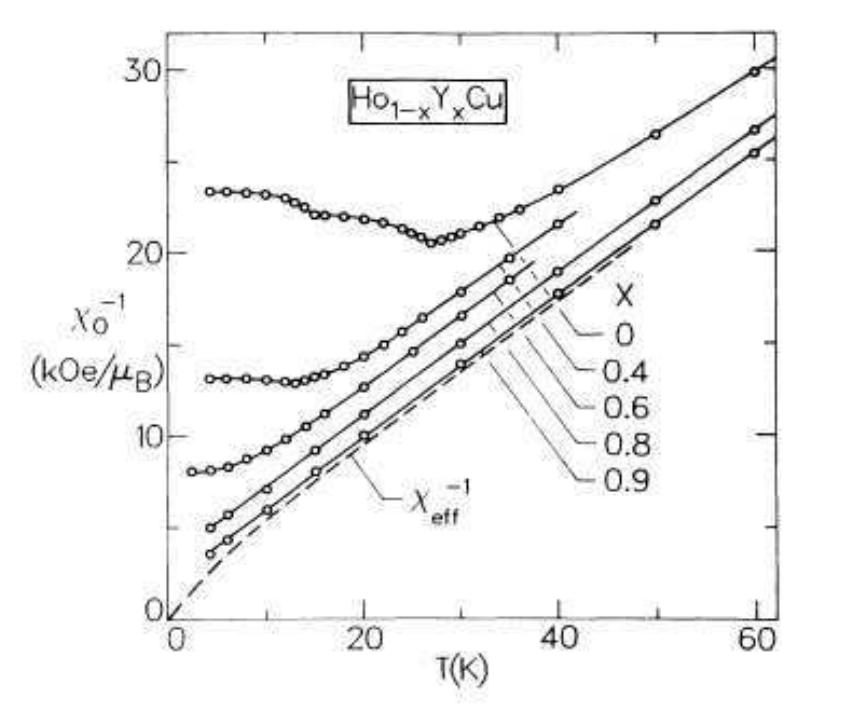
\includegraphics[scale=0.4]{SusceptibiliteMagnetique.png}
\end{center}

%\subsection{Théorie du champ cristallin}
{\sffamily\bfseries{Théorie du champ cristallin (16 points)}}

Dans un modèle plus réaliste, appelé modèle du \og champ cristallin \fg , on ajoute un terme  $A \mu_z^2$ (où $A$ est une constante caractéristique du cristal  qui peut être positive ou négative) dans l'énergie d'un ion de moment magnétique $\Vec{\mu}$ qui devient donc égale à  $A \mu_z^2 -\mu_z B$.

\question Calculer la nouvelle fonction de partition d'un seul ion $z_{CC}(T)$.

\question Calculer le moment magnétique moyen selon $(Oz)$, $M_z$, en fonction de $A, B, k_B T, N$ et $\mu$.

On travaille désormais dans la limite des champs faibles, avec $A>0$.

\question Développer $M_z$ au premier ordre en $\beta \mu B$. En déduire la susceptibilité magnétique
$\chi_M$ du cristal en champ faible. On l'exprimera en fonction de $T, k_B, N, \mu$ et \exp(\frac{3 \theta_M}{T})$ où $\theta_M=\frac{A \mu^2}{3 k_B}$.

\question Comparer $\chi_M(A >0)$ à $\chi_M(A=0)$ et interpréter.

\question 
\`A partir de l'expression de $\chi_M^{-1}$, montrer que pour $T \gg \theta_M$, $\chi_M^{-1}=\frac{T+\theta_M }{\alpha}$ et expliciter la constante $\alpha$.

\question Les mesures expérimentales de la figure sont-elles compatibles avec le résultat précédent ? Comment pourrait-on en déduire la valeur de $A$ ?

%En déduire des ordres de grandeur de $\theta_M$ et $A$ pour le composé de fraction $x=0.4$.



\section{Le modèle de Debye à deux dimensions (25 points)}
Dans un solide, chaque onde associée aux vibrations des atomes du réseau cristallin, de vecteur d'onde $\Vec{k}$ et de pulsation $\omega$, a l'énergie $\epsilon= \hbar \omega$. Ces ondes peuvent se représenter par une assemblée à nombre indéterminé (c'est-à-dire à potentiel chimique nul) de quasi-particules de nature bosonique, libres et indépendantes, appelées phonons pour lesquelles l'impulsion $\Vec{p}$ est donnée par $\Vec{p}=\hbar \Vec{k}$. Pour les petits vecteurs d'onde, ces ondes présentent des modes acoustiques dans lequel on a linéarité entre le module du vecteur d'onde et la pulsation. 

Nous considérons dans la suite le cas d'un réseau plan monoatomique de $N$ atomes à deux dimensions de longueurs $L_x$ et $L_y$. On pose $S=L_x L_y$. Il existe un mode acoustique longitudinal de célérité $c_l$ telle que $\omega = c_l k $ et un mode acoustique transversal de célérité $c_t$ telle que $\omega = c_t k $.

Le modèle de Debye consiste à attribuer à chacune des deux polarisations possibles des ondes de vibrations, des célérités respectives $c_l$ et $c_t$, constantes dans tout le domaine de variation de $k$ (et non plus aux \mbox{\og petits \fg \  $k$}). 

\question  Déterminer la densité d'état en énergie $\rho_{2D}(\epsilon)$ de ces phonons, en appliquant des conditions aux limites périodiques pour le vecteur d'onde. Montrer qu'elle est de la forme $\rho_{2D}(\epsilon)=A \epsilon$. On introduira $c$ telle que

$$\frac{2}{c^2}=\frac{1}{c_l^2}+\frac{1}{c_t^2}$$.

(En admettant le résultat $\rho_{2D}(\epsilon)=A \epsilon$, on peut poursuivre l'exercice.)

\question Le nombre total de mode de vibrations $\int \rho_{2D}(\epsilon) d\epsilon$ étant fixé à $2 N$ (2 polarisations  $\times$ $N$ particules), montrer que l'énergie d'un phonon doit avoir dans ce modèle une borne supérieure $\epsilon_D$. On introduit la température caractéristique $\Theta=\frac{\epsilon_D}{k_B}$. Relier $A$ à $N$, $\Theta$ et $k_B$.

\question \'Ecrire sous forme intégrale l'énergie interne $U$ en fonction de $N$, $\Theta, T$ et $k_B$.  Montrer que

$$U=4 N k_B \Theta \left( \frac{T}{\Theta} \right)^3  \int_0^{\frac{\Theta}{T}} \frac{x^2 dx}{e^x-1}.$$

\question \'Etudier les limites basse température ($T \ll \Theta$) et haute température ($T \gg \Theta$) de $U$. On introduira le nombre $I=\int_0^{+\infty} \frac{x^2 dx}{e^x-1}$.
 

\question En déduire les limites basse température ($T \ll \Theta$) et haute température ($T \gg \Theta$) de la capacité calorifique $C_S$. Commenter la limite obtenue à haute température. Tracer la courbe représentative de $\frac{C_S}{N k_B}$ en fonction de $\frac{T}{\Theta}$.

\question Existent-t-ils des situations physiques qui correspondent à notre modèle ?


\end{document}
\section{\'Equation d'état d'un gaz parfait selon la statistique}

La figure ci-dessous présente les équations d'état de trois gaz parfaits non relativistes à trois
dimensions (numérotées de haut en bas). Les $N$ particules de masse $m$, confinées dans un volume $V$ sont supposées sans
structure interne. Le produit $pV$ et la température $T$ sont adimensionnés grâce à la température
caractéristique : $T_0=\frac{h^2}{2\pi m k_B} \left( \frac{N}{V} \right)^{\frac{2}{3}}.$



\question
Rappeler la définition de la longueur d'onde de De Broglie $\Lambda$ à la température $T$.
Quel est son sens physique ? En déduire une interprétation de la température caractéristique $T_0$.

\question \`A quelle statistique étudiée en cours chacune de ces trois courbes correspond-elle ?

\question Expliquer l'existence d’une ordonnée à l’origine non nulle pour la courbe 1. Donner un exemple de système physique qui vérifie cette équation d'état.

\question
Concernant la courbe 3, à quel phénomène physique
la température $T^*=\frac{T_0}{\zeta(\frac{3}{2})^{\frac{2}{3}}} \approx  0,52 \ T_0$ (indiquée par un trait vertical sur la figure) correspond-elle ? $\zeta(s)=\sum_{k=1}^{+\infty} \frac{1}{k^s}$ est la fonction zêta de Riemann. 

\question Pour $T \gg T_0$, les trois courbes se rejoignent. En pratique, la courbe 2 est-elle réaliste à basse température ? Pourquoi ?

\begin{center}
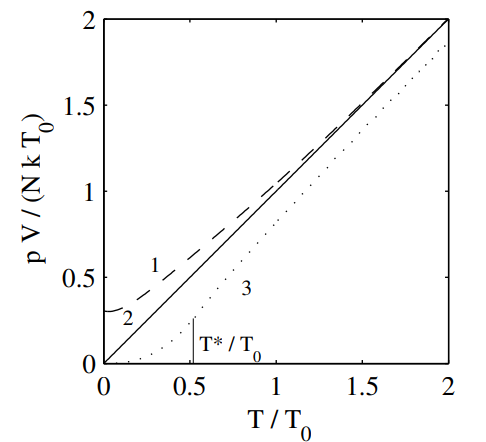
\includegraphics[scale=0.4]{TroisStatistiques.png}
\end{center}